% --------------------------------------------------
%  Week 2 – Mathematical Modeling of Disease Spread
%  Focus: Problems 4–6 (Linear stability, SIR model, Phase‑plane dynamics)
%  Version 2 (18 June 2025)
% --------------------------------------------------
\documentclass[14pt,aspectratio=169]{beamer}
\usetheme{Madrid}

% --------------------------------------------------
%          Packages
% --------------------------------------------------
\usepackage{amsmath,amsfonts,siunitx}
\usepackage{graphicx}
\usepackage{hyperref}
\usepackage[absolute,overlay]{textpos}
\definecolor{VUblue}{HTML}{002F6C}
\setbeamercolor{alerted text}{fg=VUblue}
\setbeamercolor{structure}{fg=VUblue}
% Graphics path & defaults – every figure is at most 45 % of text height
\graphicspath{{Figures/}}
\setkeys{Gin}{height=0.45\textheight,keepaspectratio}

% Textpos grid = centimetres (easier positioning)
\setlength{\TPHorizModule}{1cm}
\setlength{\TPVertModule}{1cm}

% --------------------------------------------------
%          Macros
% --------------------------------------------------
\newcommand{\dd}{\,\mathrm{d}}
\newcommand{\RR}{\mathcal{R}_0}

% --------------------------------------------------
%          Metadata
% --------------------------------------------------
\title[Modeling Disease Spread]{Key Ideas from Week 2\\Mathematical Modeling of Disease Spread}
\author{J.~Graham \and T.~Molenaar \and E.~Terjyan}
% break institute into two lines and reduce font size
\setbeamerfont{institute}{size=\footnotesize}
\institute[VU Amsterdam]{%
  Vrije University\\
  of Amsterdam \\
  Dynamical Systems Project}
\date{17 June 2025}

% --------------------------------------------------
\begin{document}

% --------------------------------------------------
\begin{frame}[plain]
    \titlepage
\end{frame}

% --------------------------------------------------
\begin{frame}{Guiding questions}
    \begin{itemize}
        \item When is the disease-free state $(S=N, \, I=0)$ stable?
        \item How does permanent immunity change outbreak dynamics? (\alert{SIR})
        \item What do phase-plane trajectories tell us about \emph{final size}?
    \end{itemize}
    \vspace{0.5em}
    \alert{Focus = Problems 4-6}
\end{frame}

% --------------------------------------------------
%   2. Linear stability of DFE
% --------------------------------------------------
\begin{frame}{Linear stability: SIS recap}
  \begin{block}{Nondimensional SIS}
    $\displaystyle s'=-\RR\,s\,i+i,\quad i'=\RR\,s\,i-i$
  \end{block}
  \begin{itemize}
    \item Disease‑free equilibrium $(s^*,i^*)=(1,0)$
    \item Jacobian eigenvalues $\lambda_1=0,\;\lambda_2=\RR-1$
  \end{itemize}
  \alert{Criterion: $\RR>1$ $\Rightarrow$ unstable $\Rightarrow$ outbreak possible.}
\end{frame}
% --------------------------------------------------
%   3. SIR model equations
% --------------------------------------------------
\begin{frame}{SIR model: adding permanent immunity}
  \begin{align*}
    \frac{\dd S}{\dd t} &= -\beta\frac{IS}{N},\\
    \frac{\dd I}{\dd t} &= \beta\frac{IS}{N}-\gamma I,\\
    \frac{\dd R}{\dd t} &= \gamma I.
  \end{align*}
  \begin{block}{Rescaled variables ($\tau=\gamma t$, $s,i,r$ are proportions)}
    $s'=-\RR s i,\; i'=\RR s i-i,\; r'=i$ \quad with \; $\RR=\beta/\gamma$
  \end{block}
  \begin{itemize}
    \item Same threshold $\RR>1$ for growth, but susceptibles deplete~$\downarrow$
    \item Trajectories live in triangle $\mathcal T:\, s\ge0,\,i\ge0,\,s+i\le1$
  \end{itemize}
\end{frame}

% --------------------------------------------------
%   4. Phase-plane portraits
% --------------------------------------------------
\begin{frame}{Phase-plane intuition}
    \centering
  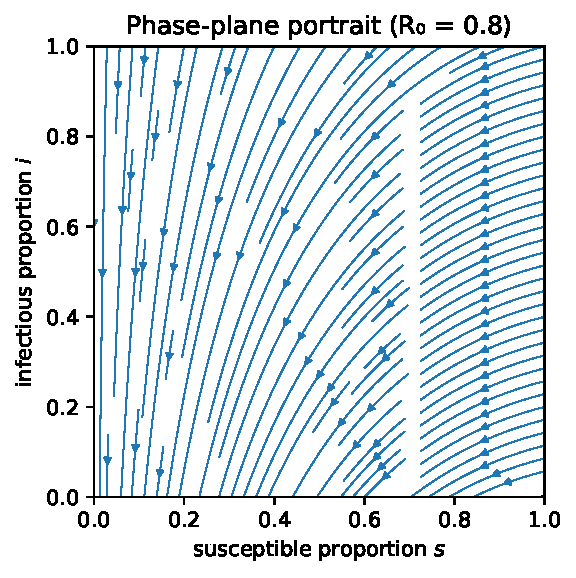
\includegraphics{PhasePlane_R0_0.8.pdf}\hfill
  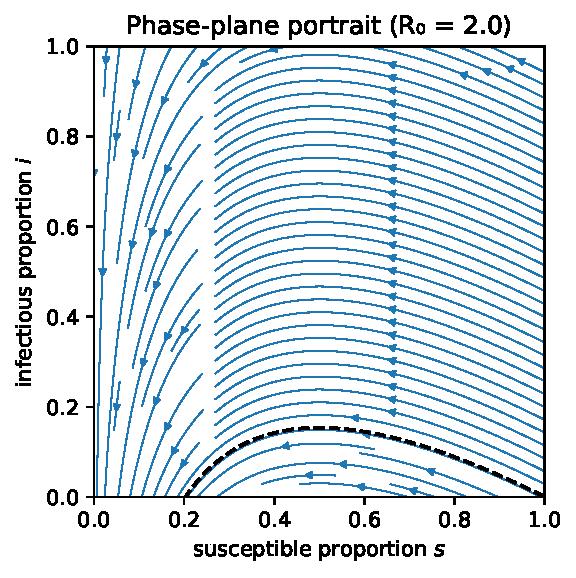
\includegraphics{PhasePlane_R0_2.0.pdf}
  \begin{textblock*}{\textwidth}(0cm,7.9cm)
    {\scriptsize Axes: \emph{susceptible proportion $s$} (horizontal) vs. \emph{infectious proportion $i$} (vertical)}
  \end{textblock*}
  \vspace{-0.15em}
  \begin{columns}[onlytextwidth]
    \column{0.48\textwidth}
      $\RR<1$ $\Rightarrow$ straight descent to DFE.
    \column{0.48\textwidth}
      $\RR>1$ $\Rightarrow$ outbreak peak then fade; final $s_\infty>0$.
  \end{columns}
\end{frame}

% --------------------------------------------------
%   5. Final‑size relation
% --------------------------------------------------
\begin{frame}{How many escape infection?}
  \begin{block}{Kermack–McKendrick integral}
    $\displaystyle \log s_\infty + \RR\,(1-s_\infty)=\log s_0$.
  \end{block}
  \begin{itemize}
    \item Implicit curve for $s_\infty$ (needs one root‑finding line!)
    \item Shows \emph{herd‑immunity payoff}: higher $\RR$ $\Rightarrow$ fewer escape.
  \end{itemize}
  \centering
  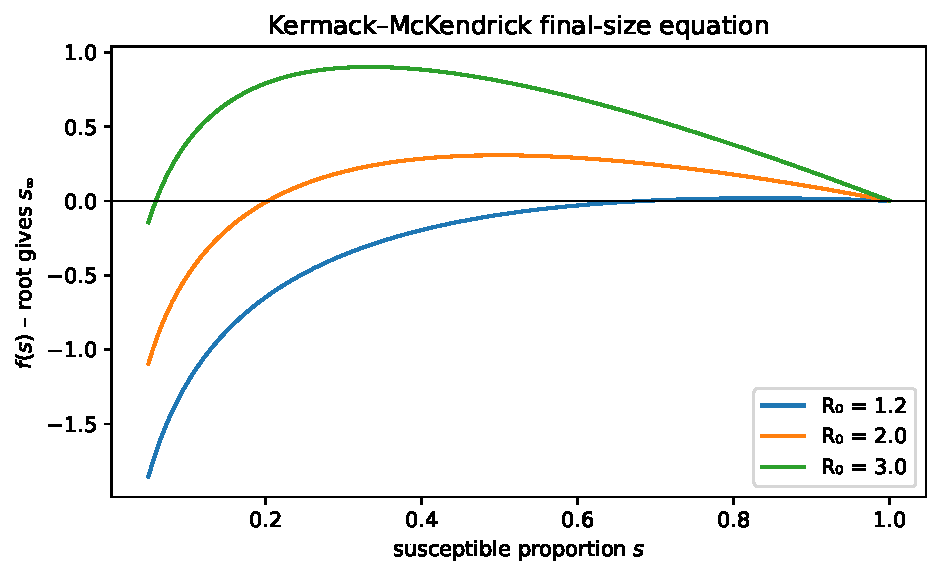
\includegraphics{FinalSizeSketch.pdf}
  \begin{textblock*}{\textwidth}(0cm,8cm)
    {\scriptsize Example curves for $s_0=0.999$ and $\RR=1.2,\,2.0,\,3.0$}
  \end{textblock*}
\end{frame}

% --------------------------------------------------
%   6. Numerical demo
% --------------------------------------------------
\begin{frame}{Numerical simulation ($\RR=2.0$)}
  \centering
  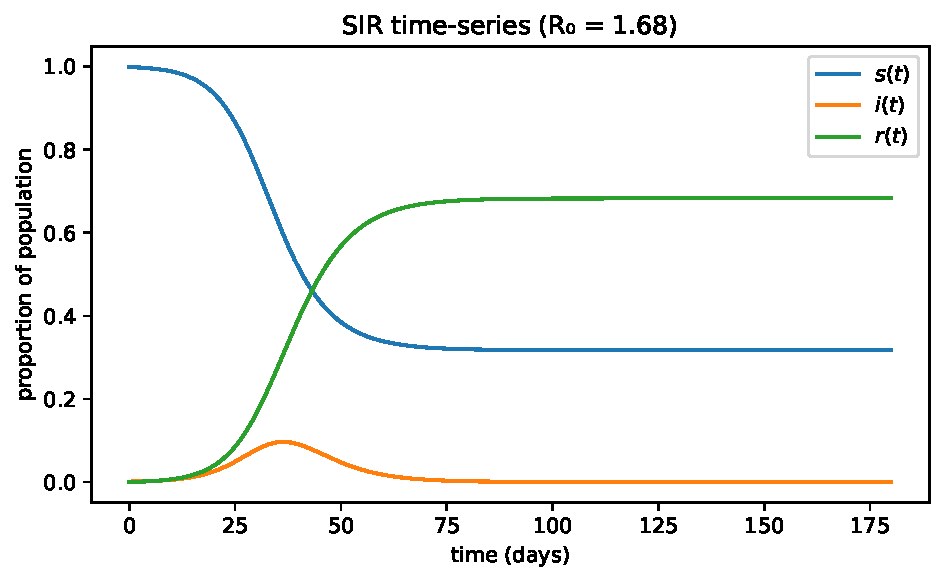
\includegraphics{SIR_Timeseries.pdf}
  \begin{textblock*}{\textwidth}(0cm,6cm)
    {\scriptsize Axes: \emph{time (days)} vs. proportions $s(t)$, $i(t)$, $r(t)$}
  \end{textblock*}
  \vspace{-0.3em}
  \begin{itemize}
    \item Peak prevalence lower than SIS (recovery + immunity).
    \item \emph{Not} everyone infected: $s_\infty\approx0.18$ in this run.
  \end{itemize}
\end{frame}
% --------------------------------------------------
%   7. Key messages
% --------------------------------------------------
\begin{frame}{Take‑aways}
  \begin{enumerate}
    \item Linearisation gives outbreak criterion: \alert{$\RR>1$}.
    \item Permanent immunity (SIR) limits outbreak – final size set by susceptible depletion.
    \item Phase‑plane view quickly communicates both threshold and final size.
  \end{enumerate}
\end{frame}

% --------------------------------------------------
%   8. Wrap‑up
% --------------------------------------------------
\begin{frame}{Conclusions \& Outlook}
  \begin{itemize}
    \item \textbf{Design implication:} vaccination reduces $s_0$ \& moves system below threshold.
    \item Next week: add births \& deaths → endemic SIRS dynamics.
    \item Code/\LaTeX:\ \href{https://github.com/ernestterjyan/mathematical_model_DS}{github.com/ernestterjyan/mathematical\_model\_DS}
  \end{itemize}
  \vfill
  \centering{\Large Thank you!}
\end{frame}

% --------------------------------------------------
% References
\begin{frame}[allowframebreaks]{References}
  \begin{thebibliography}{9}
    \bibitem{Kermack1927} W.~O.~Kermack and A.~G.~McKendrick,
      "A Contribution to the Mathematical Theory of Epidemics,"
      \textit{Proc. Roy. Soc. A}, vol.~115, pp.~700--721, 1927.
    \bibitem{Greer2018} M.~L.~Greer and D.~R.~Livesay,
      \textit{An Introduction to Mathematical Epidemiology}, Springer, 2018.
    \bibitem{Mossong2008} J.~Mossong \textit{et al.},
      "Social Contacts and Mixing Patterns Relevant to the Spread of Infectious Diseases,"
      \textit{PLoS Med.}, vol.~5, no.~3, e74, 2008.
    \bibitem{cdcYellowBook2024} Centers for Disease Control and Prevention,
      "Influenza – Travellers’ Health, CDC Yellow Book 2024," 2024.
      [Online]. Available: \url{https://wwwnc.cdc.gov/travel/yellowbook/2024/infections-diseases/influenza}
      (accessed Jun.~6, 2025).
  \end{thebibliography}
\end{frame}
\end{document}